\documentclass[conference]{IEEEtran}
%\IEEEoverridecommandlockouts
% The preceding line is only needed to identify funding in the first footnote. If that is unneeded, please comment it out.
\usepackage{cite}
\usepackage{amsmath,amssymb,amsfonts}
\usepackage{algorithmic}
\usepackage{graphicx}
\usepackage{textcomp}
\usepackage{xcolor}
\def\BibTeX{{\rm B\kern-.05em{\sc i\kern-.025em b}\kern-.08em
    T\kern-.1667em\lower.7ex\hbox{E}\kern-.125emX}}

\begin{document}

\title{ESE 2180 Project 3 Writeup}

\author{\IEEEauthorblockN{Chris Brusie}
\IEEEauthorblockA{\textit{Deptartment of Electrical Engineering} \\
\textit{Washington University in St. Louis}\\
St. Louis, United States \\
brusie@wustl.edu}
\and
\IEEEauthorblockN{Sebastian Theiler}
\IEEEauthorblockA{\textit{Deptartment of Electrical Engineering} \\
\textit{Washington University in St. Louis}\\
St. Louis, United States \\
s.k.theiler@wustl.edu}
\and
}

\maketitle


\section{Introduction}
Image processing and compression is a promising use-case of applied linear algebra. The goal of this project was to explore the use of Principle Component Analysis (PCA) for dimensionality reduction and compression of the Extended Yale B ("Eigenfaces") dataset, which consists of images of various people. Singular Value Decomposition (SVD) is applied to identify principal components, compress data, and approximate images. The report discusses methods to quantify information retention, storage reduction, and reconstruction accuracy. Results demonstrate the trade-off between feature retention and compression, providing insights into PCA's effectiveness for image analysis.

\section{Background}
PCA transforms data into a new coordinate system such that variance is maximized along orthogonal axes. Image analysis is a special case of SVD where an image with $M$ pixels is represented as a flattened vector $x_i \in \mathbb{R}^M$. The dataset contains $N$ images and is therefore represented as a matrix $X \in \mathbb{R}^{M \times N}$. PCA uses SVD to decompose $X$ into $U \Sigma V^T$, where $\Sigma$ contains singular values along its diagonals. These values quantify the variance captured by each principal component. Retaining fewer components (i.e., taking a submatrix of $\Sigma$) reduces dimensionality, enabling compression and approximation, at the cost of reduced reconstruction accuracy.

\section{Training the PCA Compression Model}
\subsection{Dataset}
The Extended Yale B, "Eigenfaces," dataset contains images of 15 individuals. 13 subjects were used for training set and two were reserved for testing. Images were resized for uniformity and flattened into a vector to construct the matrix $X$, where columns are $11368$-vectors representing images. $X$ was then demeaned by subtracting the calculated \texttt{feature\_mean}, representing an "average face", as depicted in Figure \ref{fig:feature_mean}. This results in the each column being centered on zero. This is important so that SVD can capture the variance in the data itself, rather than the shift from a non-zero mean.

\begin{verbatim}
file_list = os.listdir(folder_path)
for i, filename in enumerate(
    file_list[:num_imgs_total]
):
    img_path = os.path.join(
        folder_path,
        filename
    )
    img = cv2.imread(img_path)
    img_gray_flat = cv2.cvtColor(
        img,
        cv2.COLOR_BGR2GRAY
    ).flatten()
    img_matrix[:, i] = img_gray_flat

feature_mean = np.mean(img_matrix, axis=1)
X = img_matrix - np.outer(
  feature_mean,
  np.ones(img_matrix.shape[1])
)
\end{verbatim}

\begin{figure}[htbp]
  \centerline{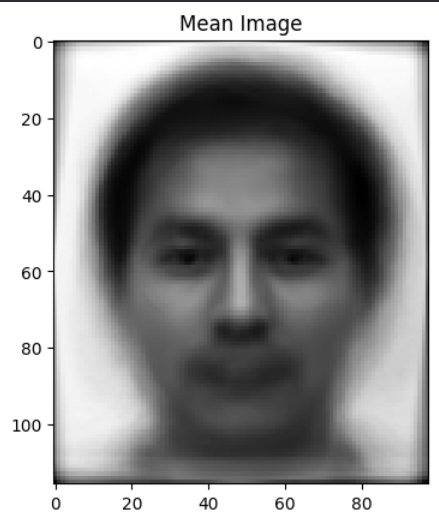
\includegraphics[scale=0.4]{figures/feature_mean.png}}
  \caption{Calculated Feature Mean representing a typical face}
  \label{fig:feature_mean}
\end{figure}  

\subsection{SVD}
SVD was performed on $X$ to extract singular values and principal components. This was done with Numpy's built-in SVD function: \texttt{U, s, Vh = np.linalg.svd(X, full\_matrices=False)}. As seen in Figure \ref{fig:svd_components}, the singular values rapidly decay for each subsequent value. The cumulative variance explained by the singular values was analyzed to determine the number of components required for 70\%, 80\%, 90\%, and 95\% data retention. These results are shown in Table \ref{tab:principal_components}.

\begin{figure}[htbp]
  \centerline{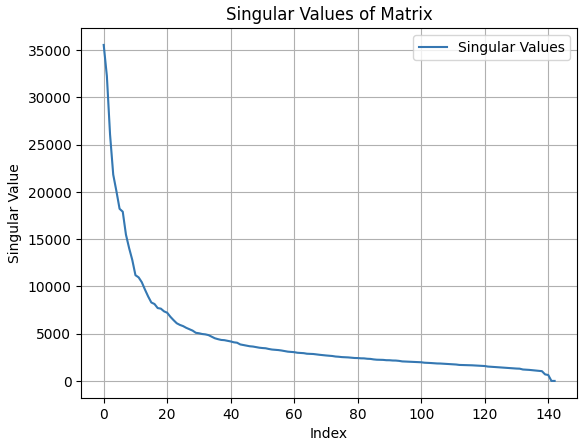
\includegraphics[scale=0.4]{figures/svd_components.png}}
  \caption{Singular Values of Matrix}
  \label{fig:svd_components}
\end{figure}  

Images were reconstructed using varying numbers of principal components $d$ ($d=20,50,70,100$), and reconstruction error was calculated as: 

\[\text{Error} = \frac{|X - \hat{X}|}{|X|}\]

where $\hat{X}$ is the approximation of $X$ using $d$ components. As seen in Figure \ref{fig:reconstructed_images}, as the number of features retained increases, the reconstructed image gradually becomes more similar to the original. Correspondingly, the error decreases from 8,200,000 with $d=20$ to 680,000 with $100$.


\begin{table}[h!]
\centering
\begin{tabular}{|c|c|}
\hline
\textbf{Accuracy Level} & \textbf{Principal Components Needed} \\ \hline
95\%                     & 59                                   \\ \hline
90\%                     & 34                                   \\ \hline
80\%                     & 16                                   \\ \hline
70\%                     & 10                                   \\ \hline
\end{tabular}
\caption{Principal Components Needed for Different Accuracy Levels}
\label{tab:principal_components}
\end{table}


\begin{figure}[htbp]
  \centerline{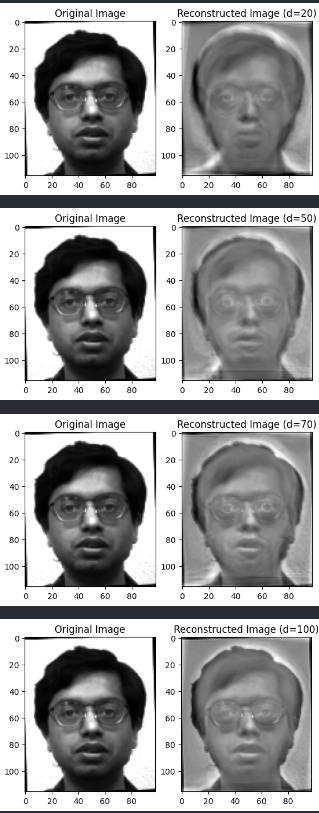
\includegraphics[scale=0.4]{figures/reconstructed_images.png}}
  \caption{Reconstructed Images of Sample 100 for $d=20,50,70,100$}
  \label{fig:reconstructed_images}
\end{figure}  

\section{Compressing Test Data}
Finally, using 50 principal components from the training data, test images from two subjects were approximated.
\begin{verbatim}
d = 50
U_50 = U[:, :d]
projections = U_50.T @ X_test
test_reconstruct = U_50 @ projections + \
    np.outer(
        np.mean(img_matrix_test, axis = 1),
        np.ones(img_matrix_test.shape[1])
)
\end{verbatim}

Reconstruction error was measured for these test images. One of the test images is depicted in Figure \ref{fig:reconstructed_test}. On average, the test images had an error of 230,000,000, which is considerably higher than the error of 3,100,000 for the equivalent number of features on the testing dataset. This is reasonable as the PCA values were not trained on this particular faces. Additionally, reconstruction was evaluated on a rotated image ('subject15rotated.jpeg'), depicted in Figure \ref{fig:reconstructed_rotated}. The reconstructed image visibly loses most detail and is essentially unrecognizable, with an error of 603,000,000.

\begin{figure}[htbp]
  \centerline{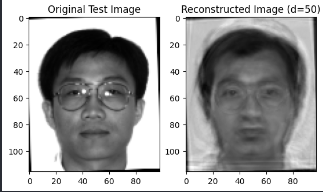
\includegraphics[scale=0.4]{figures/reconstructed_test.png}}
  \caption{Reconstructed Image of a Testing Example}
  \label{fig:reconstructed_test}
\end{figure}  

\begin{figure}[htbp]
  \centerline{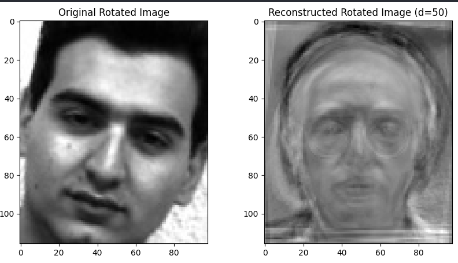
\includegraphics[scale=0.4]{figures/reconstructed_rotated.png}}
  \caption{Reconstruction of a Rotated Image}
  \label{fig:reconstructed_rotated}
\end{figure}  

\section{Discussion and Conclusion}
This study demonstrates PCA's ability to reduce the dimensionality of high-dimensional image data while preserving significant detail. The results indicate that a comparatively small number of principal components can capture a large percentage of the variance, enabling for the preservation of a high resolution image with a substantial reduction in storage. For example, with only 10 features, 70\% of the variance can be accounted for. While the compression of images proves to be useful across many engineering disciplines, if not done efficiently, it can severely distort the given image, resulting in a loss of discernable features. In this project, the program was able to successfully decrease the dimensionality and maintain a relatively comprehensible image. The images did endure a considerable amount of alteration from the compression, however, key details were conserved and a resemblance was present between the resulting and the input images. This is to be expected, as it would be essentially impossible to compress the original image vector while substaining zero image distortion. Furthermore, PCA's performance is contingent on the training data's representativeness. The considerably increased error observed with the rotated image highlights PCA's limitation in handling variations not present during training. Future work could explore incorporating additional transformations in the training set or employing more robust dimensionality reduction techniques to enhance invariance. Despite this, PCA remains a valuable tool in scenarios where efficient compression and approximate reconstructions are acceptable, such as facial recognition or large-scale image datasets.

%\begin{thebibliography}{00}
%
%\bibitem{spanishflu}
%Cleveland clinic, 2021, “Spanish Flu: What Is It, Causes, Symptoms \& Pandemic,” Cleveland Clinic, Sep. 21, 2021. Available: https://my.clevelandclinic.org/health/diseases/21777-spanish-flu
%
%\bibitem{b1} 
%World Health Organization, 2021, "The True Death Toll of COVID-19: Estimating Global Excess Mortality," World Health Organization, May. Available: https://www.who.int/data/stories/the-true-death-toll-of-covid-19-estimating-global-excess-mortality
%
%\bibitem{b2} 
%United States Census Bureau, 2021, "Census Regions and Divisions of the United States," United States Census Bureau. Available: https://www.census.gov/geographies/reference-maps/2020/geo/division.html
%
%\bibitem{walmart}
%Walmart, 2024, “Mezorrison KN95 Face Masks, 50-Pack, Black,” Walmart. Available: https://www.walmart.com/ip/Mezorrison-KN95-Face-Masks-50-Pack-Black/518596184?classType=VARIANT
%
%\end{thebibliography}

\end{document}
